% !TeX root = ../main.tex

\chapter{Results}\label{chapter:results}

\section{Data}
A total of 6 users clicked the access link and registered in the system.
The users have collectively logged a total of 150 entries by 14/07/2019.
Distribution of these entries among users can be seen in \autoref{fig:user-entry}.

\begin{figure}[htbp]
  \centering
  \captionsetup{width=.9\linewidth}
  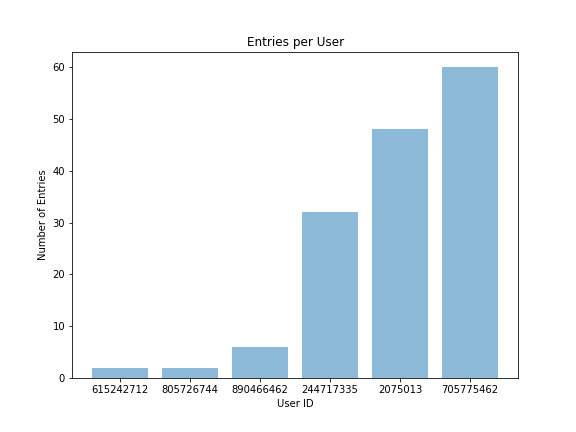
\includegraphics[scale=0.6]{figures/user-entry}
  \caption{Distribution of Entries per User}
  \label{fig:user-entry}
\end{figure}

After removing the users with less than 10 entries, we are left with 3 users.
Eating patterns of these 3 users can be seen in \autoref{fig:user-pattern}.

\begin{figure}[htbp]
  \centering
  \captionsetup{width=.9\linewidth}
  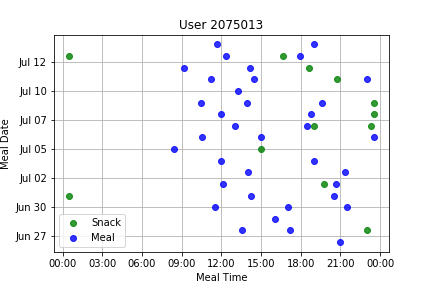
\includegraphics[scale=0.6]{figures/2075013_pattern}
  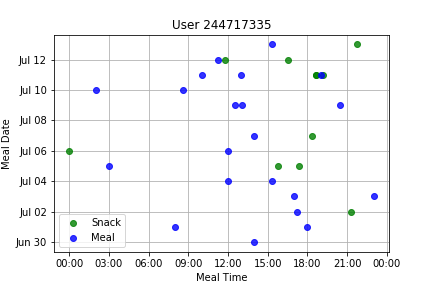
\includegraphics[scale=0.6]{figures/244717335_pattern}
  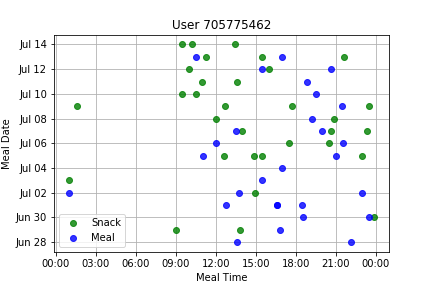
\includegraphics[scale=0.6]{figures/705775462_pattern}
  \caption{Eating Patterns of the Most Active Three Users}
  \label{fig:user-pattern}
\end{figure}

\newpage
\section{Models}
Best scoring models and the corresponding $R^2$ scores for the users with more than 10 entries can be seen in \autoref{fig:user-model}.
\begin{figure}[htbp]
  \centering
  \captionsetup{width=.9\linewidth}
  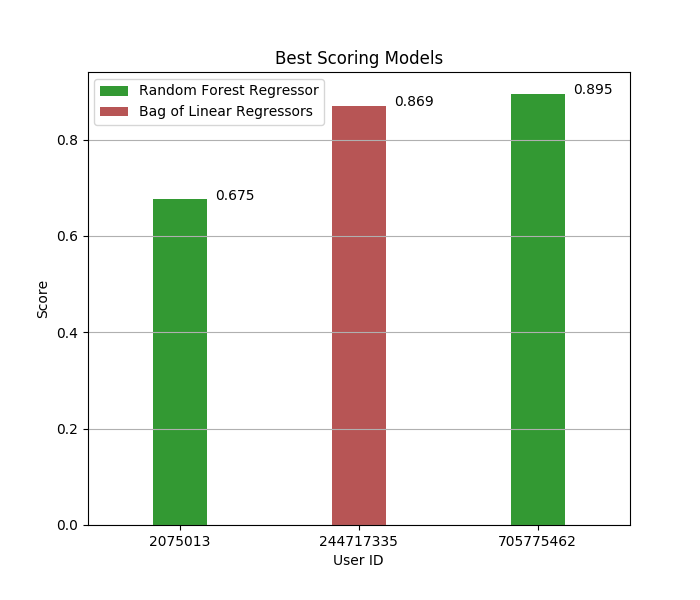
\includegraphics[scale=0.6]{figures/user-model}
  \caption{Best Scoring Models and the Corrosponding $R^2$ Scores}
  \label{fig:user-model}
\end{figure}


